\documentclass[11pt]{article}

\usepackage{xcolor}
\usepackage{caption}
\usepackage{amsmath}
\usepackage{graphicx}
\usepackage{hyperref}
\usepackage{tabularx}
\usepackage{listings}
\usepackage{tcolorbox}
\usepackage[utf8]{inputenc}
\usepackage[margin=20mm]{geometry}

\definecolor{codegreen}{rgb}{0,0.6,0}
\definecolor{codegray}{rgb}{0.5,0.5,0.5}
\definecolor{codepurple}{rgb}{0.58,0,0.82}

\lstdefinestyle{simplecode}{
    commentstyle=\color{codegreen},
    keywordstyle=\color{magenta},
    numberstyle=\tiny\color{codegray},
    stringstyle=\color{codepurple},
    basicstyle=\ttfamily\footnotesize,
    breakatwhitespace=false,         
    breaklines=true,                 
    captionpos=b,                    
    keepspaces=true,                 
    %numbers=left,                    
    numbersep=5pt,                  
    showspaces=false,                
    showstringspaces=false,
    showtabs=false,                  
    tabsize=2
}

\lstset{style=simplecode}


% ----- END OF PREAMBLE -----




\title{Real-Time Scheduling: Project Report}
\author{Sampreet Sarkar\footnote{M2 Control and Robotics: Embedded Real-Time Systems, \textit{\'Ecole Centrale de Nantes}}}
\date{}

\begin{document}
\nocite{*}
\maketitle

\section{Introduction}
The goal of this project is to simulate the behaviour of a Preemptive Fixed-Priority Scheduler\textit{(Rate Monotonic)}. We shall move along with the assumption that all the tasks are periodic, with the task deadline equal to the task period. The design of the software will be detailed in the following sections, along with the accompanying source code, which can be found in the appendix.\\

A scheduler is an extremely important part of any Operating System, as it is in charge of breaking up tasks into jobs and executing them in a particular order to maintain the illusion of pseudo-parallelism that we commonly associate with the term \texttt{"multitasking"}. This behaviour becomes doubly important in the case of a Real-Time Operating System, because in addition to executing tasks correctly, the scheduler has to also keep in mind to return results on time, otherwise the result of the computation is invalid, and cannot be used for any good purpose.\\

Before we begin to describe the common functionalities and the design of the software, it is imperative that we take a look into the programming paradigm being followed in the development of the scheduler. The core of the scheduler has been implemented in the C++ language, which although is a close second choice of language for developping embedded applications, provides a fast enough speed and above all, embodies the use of STL classes and Object-Oriented Programming benefits. The STL template classes \textit{(especially vector and algorithm)} provide us with many helper functions, which make our life easier. Another choice to justify C++ as the optimal language of choice for this particular project is due to the innumerable open-sourced libraries that are available for the language, which lets the user accomplish a lot of complicated programming in a matter of minutes. The final executables are generated by the CMake\cite{cmake} tool, which allows us to automate the build process and give our software a little more polish. The version control is done using Git, and the online repository for the project can be found \href{https://github.com/sampreets3/scheduler-RM}{here}.\\

In the upcoming sections, we will discuss four main aspects of a scheduler|\textit{viz.}, data acquisiton, schedulability analysis, simulation of the schedule, and evaluation of the metrics. The \texttt{data acquisition} section will deal with the general idea of how to represent the contents of a simulated task to our scheduler, the \texttt{schedulability analysis} will deal with running several schedulability tests on the set of tasks in order to determine whether a given taskset is indeed schedulable or not, the \texttt{simulation} of the schedule would ideally include some representation of how the scheduling algorithm places jobs at each time instant, and the \texttt{metrics} we would want to evaluate will give us a benchmark to compare the performance of our algorithm against other solutions. Some of the metrics that define the efficiency of a scheduler is the number of context switches, the maximum idle time for the processor, and the average response time for each task.

\section{Data Acquisition}\label{sec:data-acquisition}

In this section, we are interested in obtaining the data from a simulated task, and generating our taskset $\tau$ from this data. If we think in terms of the \textit{(simulated)}scheduler, the only information we need about a task are its identifier, the computation time, the period, and the deadline of the task. Since it has already been established that in our case, the period is equal to the deadline, we can make do with either information. We also understand that we would need some kind of data structure to contain this information in an easily-retrievable fashion. Thus, we can utilize a data structure as shown in Fig. \ref{fig:tcb} below:

\begin{figure}[h!]
  \centering
  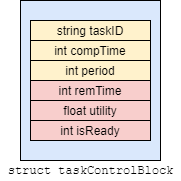
\includegraphics[scale=0.5]{../imgs/single-tcb}
  \caption{Data structure of a single task control block}
  \label{fig:tcb}
\end{figure}

We also notice that we have some extra fields in our data structure, namely \texttt{remTime}, \texttt{utility}, and \texttt{isReady}. These are not assigned by the user, but are really important to carry out the scheduling of the taskset. Here, the variable remTime stores the remaining execution time of the task, utility stores the utility of the task, and isReady is a flag that denotes the state of the task.\\

With all this information at hand, we can go ahead and create our data structure as denoted in the code listing  below. In order to increase readability, we have distributed the entirety of the code into specialised header and source files, each of which provide some special functionality to the entire software. As a result of this distributed approach, one would find it extremely easy to navigate through specific section of code, to better understand the functionality or to modify it according to the development need.

\lstinputlisting[language=c, firstline=6, lastline=16]{../../lib/tasks.hpp}

You will also observe that we have created a vector of these data structures, so that when a new task is created, the equiavalent taskControlBlock can be pushed into this vector. This will allow us to perform various vector based operations on the taskset\textit{(sorting, pushing at the tail, getting the size)} which have already been defined in the C++ STL \texttt{<vector>}.\\

Moving forward, we would like to facilitate the user's process of creating a task. For this purpose, we propose the function \texttt{createTask()}, which will allow us to create a new taskControlBlock element, and push it into the list of tasks. The implementation of the function can be seen in the following code listing\footnote{The main inspiration behind the nomenclature of the functions has been Trampoline, as it is a very elegantly designed RTOS, and since we already had some prior exposure to the functionalities.}:

\lstinputlisting[language=c, firstline=10, lastline=21]{../../src/tasks.cpp}

We have thus been able to devise a way for the user to define a task to be scheduled. Note that unlike other Fixed-Priority schedulers, we do not ask for a priority level from the user, we get around this by simply taking the size of the taskset as the maximum priority level, and ordering our taskControlBlock elements within the vector in ascending order of period. This saves us from having to validate user input, and lets us abstract the concept of priority assignment from the user.\\

In the upcoming section, we will focus on performing rigorous schedulability tests on a populated taskset, and let the user know if the schedule is indeed feasible or not.

\section{Schedulability Analysis}\label{sec:sched-analysis}

Our goal in this section is to provide an insight to the feasability of a taskset. In order to do this, we must understand the conditions for schedulability of a taskset, laid out by Liu and Layland\cite{liu-layland}. There are two conditions, the sufficient condition and the necessary condition.\\

\begin{tcolorbox}[title=Necessary Scheduling Condition]
A taskset $\tau$ is schedulable by a Rate-Monotonic scheduler if and only if:
\begin{equation}
  U \leq 1
\end{equation}
Where $U$ is the total processor utilisation.
\end{tcolorbox}

\begin{tcolorbox}[title=Sufficient Scheduling Condition]
A taskset $\tau$ is schedulable by a Rate-Monotonic scheduler if and only if:
\begin{equation}\label{eqn:sufficient-condition}
  U \leq n({2}^{\frac{1}{n}} - 1)
\end{equation}

Where $U$ is the total processor utilisation, and $n$ is the number of tasks in the taskset $\tau$.
\end{tcolorbox}

From the equation \ref{eqn:sufficient-condition}, we observe that the as the number of tasks increase, the value of $n({2}^{\frac{1}{n}} - 1)$ converges to $ln(2) = 0.693$. Thus, we can make an inference that the rate monotonic scheduler is not the best algorithm for maximising the processor usage. It is however, extremely deterministic in its functioning, which is why it is a widely used scheduler for mission-critical systems.\\

Now, let us take an example taskset and try to perform these checks to determine whether the taskset will be feasible or not. This is done in order to "think in terms of the scheduler", and will eventually help us design the algorithm. Consider the following taskset $\tau$\footnote{$\tau$ can also be represented in a more compact fashion as follows: $\tau = \left[(T_{1}, 1, 8), (T_{2}, 2, 5), (T_{3}, 2, 10) \right] $}:
\begin{center}
\begin{tabular}{|c|c|c|}
  \hline
  Task & Computation Time & Period \\
  \hline
  T1 & 1 & 8 \\
  \hline
  T2 & 2 & 5 \\
  \hline
  T3 & 2 & 10 \\
  \hline
\end{tabular}
\end{center}

Assuming that the deadline for each task is equal to the period, we can proceed to checking whether this taskset $\tau$ is indeed feasible or not. We begin by computing the total processor utilisation $U$, which is calculated as:

\begin{equation} \label{eqn:proc-util-calc}
\begin{split}
U & = \sum_{i=1}^{3}\frac{C_{i}}{T_{i}} \\
  & = \frac{1}{8} + \frac{2}{5} + \frac{2}{10} \\
  & = \frac{29}{40} \\
  & = 0.725
\end{split}
\end{equation}
As we see that the value of U is less than 1, we can say that the necessary condition has been verified. This lets us know that the taskset might be feasible. We need to further verify this claim by checking the sufficient condition check, calculated as follows:
\begin{equation} \label{eqn:suf-test-calc}
\begin{split}
n({2}^{\frac{1}{n}} - 1) & = 3({2}^{\frac{1}{3}} - 1) \\
                         & = 3(1.259 - 1) \\
                         & = 3(0.259) \\
                         & = 0.777
\end{split}
\end{equation}
As we see that the total processor utilisation\textit{(from eqn.\ref{eqn:proc-util-calc})} is lesser than 0.777, we can say that the taskset $\tau$ is schedulable. Now if we want to figure out the schedule, we need to focus on the algorithm, presented as follows:\\

\begin{tcolorbox}[title=Rate-Monotonic Scheduling Algorithm]
  The task with the lowest period is scheduled first, and then the task with the next lowest period is scheduled. Preemption occurs
  when a low priority task is scheduling and a higher priority task is released.
\end{tcolorbox}
\vspace{5mm}
If we follow this algorithm, we can obtain the schedule as follows:
\begin{figure}[!ht]
  \centering
  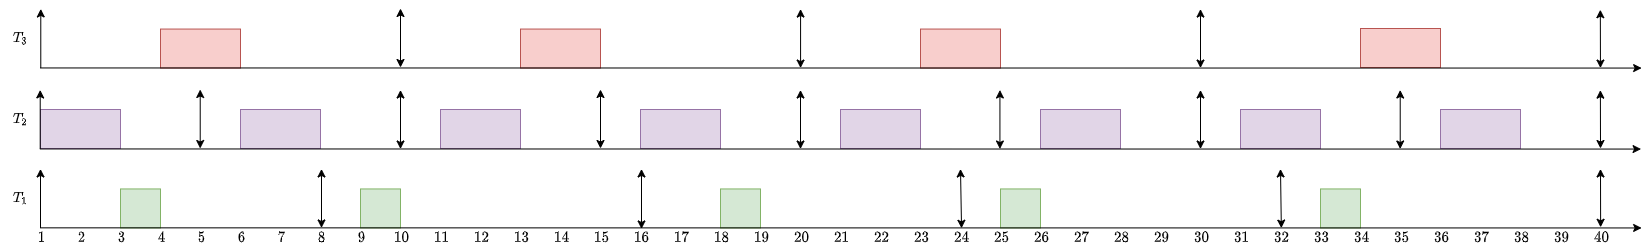
\includegraphics[width=\textwidth]{../imgs/sched-analysis}
  \caption{Feasible schedule of the taskset $\tau$}
\end{figure}

These conditions can be very easy to be implement in code, as we can harvest all of the important information from the task control block or the taskset itself. During the writing of the software, we found it was more convenient to include an additional field for storing the remaining execution time and the utility of the task itself. This would allow for lesser computations overall, hence making our program more efficient.\\

In the next section, we will see the scheduler simulate three different task sets, and we will see a few limitations of the software and the scheduling algorithm itself.

\section{Simulation Results}\label{sec:sim-results}
The scheduled task set will be simulated from time zero to the first hyperperiod of the task set. We simulate only up till the first hyperperiod because the behaviour of the system is cyclic with respect to the hyperperiod, \textit{i.e.}, the same schedule will be repeated each hyperperiod. We will simulate three use cases to understand the design and capabilities of the software. We will have our first taskset which can be scheduled without any conflict by the scheduler, then we will see a second taskset which the scheduler will not be able to schedule and for the final simulation, we will carefully choose a taskset which we know is schedulable, but the scheduler will say it is not, thus showing the limitations of such a scheduler.\\
\subsection{Case I: Taskset scheduled without any conflict}

In this section, we will simulate a simple taskset that will be schedulable by the scheduler after having passed both the schedulability tests. Consider the following taskset $\tau$:
\begin{center}
\begin{tabular}{|c|c|c|}
  \hline
  Task & Computation Time & Period \\
  \hline
  T1 & 2 & 8 \\
  \hline
  T2 & 4 & 16 \\
  \hline
  T3 & 1 & 4 \\
  \hline
\end{tabular}
\end{center}

We can observe the output of the program and the schedule in the following figures \ref{fig:case1-output} and \ref{fig:case1-schedule} respectively.

\begin{figure}[!ht]
\centering
\begin{minipage}{.5\textwidth}
  \centering
  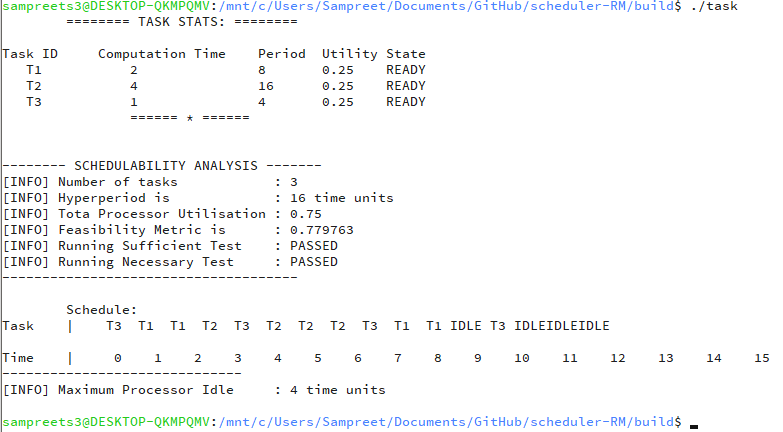
\includegraphics[width=\linewidth]{../imgs/sim-case1-output}
  \captionof{figure}{The program output on taskset $\tau$}
  \label{fig:case1-output}
\end{minipage}%
\begin{minipage}{.5\textwidth}
  \centering
  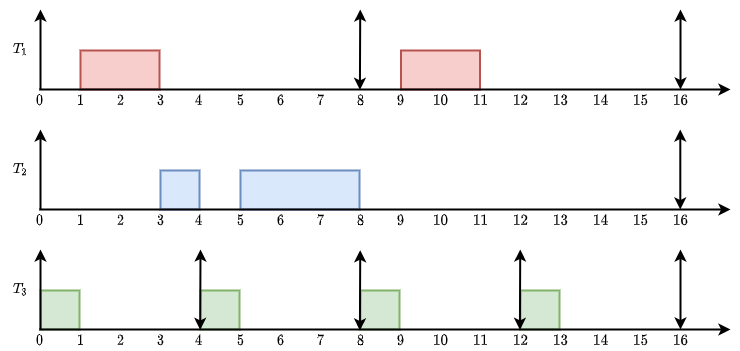
\includegraphics[width=\linewidth]{../imgs/sim-case1-schedule}
  \captionof{figure}{The produced schedule}
  \label{fig:case1-schedule}
\end{minipage}
\end{figure}

\subsection{Case II: Taskset Not Schedulable}

Our aim in this case is to provide the scheduler with an unschedulable taskset, and see if it can effectively reproduce the results, \textit{i.e.,} let us know that the taskset is not schedulable. We will take a simple example so that it is easy to study by hand as well. Consider the following taskset $\tau$:
\begin{center}
\begin{tabular}{|c|c|c|}
  \hline
  Task & Computation Time & Period \\
  \hline
  T1 & 3 & 10 \\
  \hline
  T2 & 2 & 4 \\
  \hline
  T3 & 3 & 6 \\
  \hline
\end{tabular}
\end{center}

We can deduce by looking at the taskset that it is not going to be schedulable, as the total processor utilisation $U$ is $1.3$, which is greater than the upper bound of 1. We will now observe the output of the program to verify our results.

\begin{figure}[h!]
\centering
  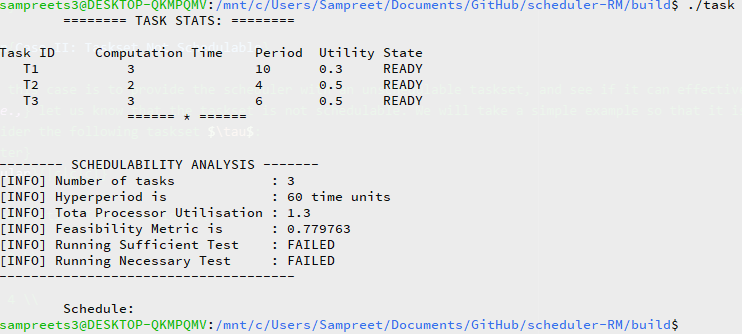
\includegraphics[scale=0.75]{../imgs/sim-case-2-output}
  \caption{Simulation of the taskset $\tau$, which is not schedulable.}
\end{figure}

\subsection{Case III: Taskset scheduled with conflict}

This is a particularly interesting case, where we can observe that although the taskset does not pass any of the schedulability tests, the taskset is indeed scheduled by our scheduler. This highlights the integgrity and the flexibility of the software we have written.\\

Consider the following taskset $\tau$:
\begin{center}
\begin{tabular}{|c|c|c|}
  \hline
  Task & Computation Time & Period \\
  \hline
  T1 & 1 & 2 \\
  \hline
  T2 & 1 & 4 \\
  \hline
  T3 & 2 & 8 \\
  \hline
\end{tabular}
\end{center}

We can observe from the taskset that the total processor utilisation here will be 1. This will cause the necessary and sufficient conditions to fail. However, when we run the program, we will see that it indeed produces a schedule which is feasible. This goes on to show that our scheduler tries to fit in the taskset to the best of its abilities. Note that this schedule is incomplete of information, we will need to know if there are any shared resources, and how they interact with each other to know the blocking time. This will let us know whether the taskset is indeed schedulable or not.

\begin{figure}[!ht]
\centering
\begin{minipage}{.5\textwidth}
  \centering
  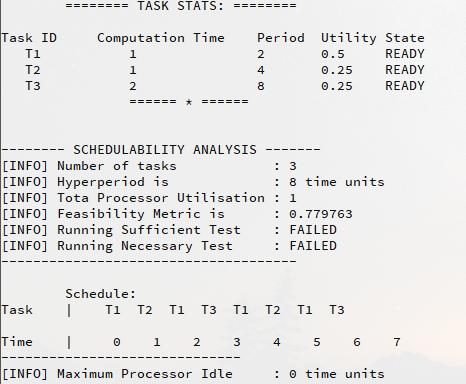
\includegraphics[width=\linewidth]{../imgs/sim-test3}
  \captionof{figure}{The program output on taskset $\tau$}
  \label{fig:case3-output}
\end{minipage}%
\begin{minipage}{.5\textwidth}
  \centering
  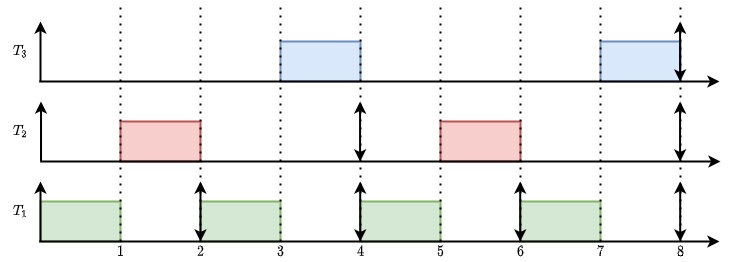
\includegraphics[width=\linewidth]{../imgs/sim-result-case-3}
  \captionof{figure}{The produced schedule}
  \label{fig:case3-schedule}
\end{minipage}
\end{figure}
\pagebreak
\section{Evaluation of Main Metrics}\label{sec:main-metrics}
 In this section we will evaluate the main metrics for the scheduler. This will give us more information about the performance of each task during the scheduling.\\

 We will see in the code the following evaluation of metrics:
 \begin{itemize}

  \item \begin{equation}
          \mbox{Number of Releases, } N_i = \frac{Hyperperiod(\tau)}{Period(\tau_{i})} \forall\;\tau_{i} \in \;\tau
        \end{equation}

 \item \begin{equation}
          \mbox{Total Idle Time, } T_{idle} = Hyperperiod(\tau) - (U \cdot Hyperperiod(\tau))
       \end{equation}

 \item
      \begin{equation}
            \mbox{Release Time, }R_i = j \cdot \mbox{Period}(i), \;\;\;\forall \;i \in \mbox{ Number of tasks in }\tau
       \end{equation}

  \item
      \begin{equation}
          \mbox{Waiting Time, } W_i = \mbox{Start Time}(\tau_i) - \mbox{Release Time}(\tau_i)
      \end{equation}
\end{itemize}

These metrics have been evaluated using a simple function, called \texttt{evaluateMetrics}, a part of which is shown in the listing below:
\lstinputlisting[language=c, firstline=15, lastline=33]{../../lib/scheduler.hpp}

\section{Conclusion}
The aim of this project was to gain an understanding about how a rate-monotonic scheduler functions. We have been able to explore the core principles of a Fixed-Priority Rate Monotonic Scheduler in some detail, where we saw how we can conceptualise a simple task control block, how to store this information in a structured format, and how to facilitate creation, addition, deletion, and sorting of the tasks internally with the list of tasks using C++ STL classes.\\

In the next section, we gained insight on how we would acquire data for our scheduler, highlighting the branching out of source code into multiple files, enabling file input/output, and in general giving it a more application feel. Once we had acquired the data, we wanted to check if the taskset was indeed feasible or not before trying to compute a schedule for it. For this purpose, we made use of the necessary and sufficient schedulability checks, and learnt how to compute them by solving an example by ourselves.\\

Finally, when the schedule had been computed, we had to display the main metrics and evaluate our scheduler against the rest of the schedulers out there. We saw a very simple method of comparision, and how we can achieve that in code.\\

As far as proposed updates are concerned, the popular plotting library matplotlib will be included in order to directly provide the GANTT diagrams. Work is also underway with extrapolation of this software to incorporate multi-processor based scheduling.\\

Overall, it was an extremely enriching experience, which has helped us understand not only the basics of rate monotonic scheduling, but also about software development practices in general.

\bibliographystyle{unsrt}
\bibliography{references.bib}

\pagebreak
\section*{Appendix}
\documentclass[11pt]{article}

\usepackage{xcolor}
\usepackage{graphicx}
\usepackage{listings}
\usepackage{tcolorbox}
\usepackage[utf8]{inputenc}
\usepackage[margin=15mm]{geometry}

%\tcbuselibrary{skins,breakable}

\definecolor{codegreen}{rgb}{0,0.6,0}
\definecolor{codegray}{rgb}{0.5,0.5,0.5}
\definecolor{codepurple}{rgb}{0.58,0,0.82}

\lstdefinestyle{simplecode}{
    commentstyle=\color{codegreen},
    keywordstyle=\color{magenta},
    numberstyle=\tiny\color{codegray},
    stringstyle=\color{codepurple},
    basicstyle=\ttfamily\footnotesize,
    breakatwhitespace=false,
    breaklines=true,
    captionpos=b,
    keepspaces=true,
    %numbers=left,
    numbersep=5pt,
    showspaces=false,
    showstringspaces=false,
    showtabs=false,
    tabsize=2
}

\lstset{style=simplecode}

\begin{document}

\section*{Code listing for the software}

The entire source code is split up into multiple files, which are orgainised in the following manner:
\begin{figure}[h!]
	\centering
	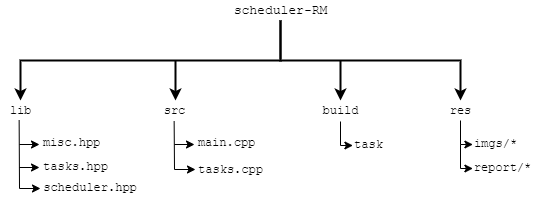
\includegraphics[scale=0.65]{imgs/hierarchy}
\end{figure}


\begin{tcolorbox}[title=\textbf{main.cpp}: This is the main application which the user will interact with.]
\lstinputlisting[language=c]{../src/main.cpp}
\end{tcolorbox}


\begin{tcolorbox}[title=\textbf{tasks.hpp} : This file contains the definition for the taskControlBlock structure and various functions that pertains to the manipulation of a task.]
\lstinputlisting[language=c]{../lib/tasks.hpp}
\end{tcolorbox}

\begin{tcolorbox}[title=\textbf{tasks.cpp} : This file contains the source code for the functions defined in \texttt{lib/tasks.hpp}]
\lstinputlisting[language=c]{../src/tasks.cpp}
\end{tcolorbox}

\begin{tcolorbox}[title=\textbf{misc.hpp}: This is a small file with helper functions pertaining to a more general use case.]
\lstinputlisting[language=c]{../lib/misc.hpp}
\end{tcolorbox}

\begin{tcolorbox}[title=\textbf{scheduler.hpp}: This file contains all the important functions and parameters related to the scheduler.]
\lstinputlisting[language=c, firstline=1, lastline=54]{../lib/scheduler.hpp}
\end{tcolorbox}

\begin{tcolorbox}[title=\textbf{scheduler.hpp}\textit{(contd.)}]
\lstinputlisting[language=c, firstline=55]{../lib/scheduler.hpp}
\end{tcolorbox}

\end{document}

\end{document}
